% Options for packages loaded elsewhere
\PassOptionsToPackage{unicode}{hyperref}
\PassOptionsToPackage{hyphens}{url}
\PassOptionsToPackage{dvipsnames,svgnames,x11names}{xcolor}
%
\documentclass[
  letterpaper,
  DIV=11,
  numbers=noendperiod]{scrartcl}

\usepackage{amsmath,amssymb}
\usepackage{iftex}
\ifPDFTeX
  \usepackage[T1]{fontenc}
  \usepackage[utf8]{inputenc}
  \usepackage{textcomp} % provide euro and other symbols
\else % if luatex or xetex
  \usepackage{unicode-math}
  \defaultfontfeatures{Scale=MatchLowercase}
  \defaultfontfeatures[\rmfamily]{Ligatures=TeX,Scale=1}
\fi
\usepackage{lmodern}
\ifPDFTeX\else  
    % xetex/luatex font selection
\fi
% Use upquote if available, for straight quotes in verbatim environments
\IfFileExists{upquote.sty}{\usepackage{upquote}}{}
\IfFileExists{microtype.sty}{% use microtype if available
  \usepackage[]{microtype}
  \UseMicrotypeSet[protrusion]{basicmath} % disable protrusion for tt fonts
}{}
\makeatletter
\@ifundefined{KOMAClassName}{% if non-KOMA class
  \IfFileExists{parskip.sty}{%
    \usepackage{parskip}
  }{% else
    \setlength{\parindent}{0pt}
    \setlength{\parskip}{6pt plus 2pt minus 1pt}}
}{% if KOMA class
  \KOMAoptions{parskip=half}}
\makeatother
\usepackage{xcolor}
\setlength{\emergencystretch}{3em} % prevent overfull lines
\setcounter{secnumdepth}{-\maxdimen} % remove section numbering
% Make \paragraph and \subparagraph free-standing
\makeatletter
\ifx\paragraph\undefined\else
  \let\oldparagraph\paragraph
  \renewcommand{\paragraph}{
    \@ifstar
      \xxxParagraphStar
      \xxxParagraphNoStar
  }
  \newcommand{\xxxParagraphStar}[1]{\oldparagraph*{#1}\mbox{}}
  \newcommand{\xxxParagraphNoStar}[1]{\oldparagraph{#1}\mbox{}}
\fi
\ifx\subparagraph\undefined\else
  \let\oldsubparagraph\subparagraph
  \renewcommand{\subparagraph}{
    \@ifstar
      \xxxSubParagraphStar
      \xxxSubParagraphNoStar
  }
  \newcommand{\xxxSubParagraphStar}[1]{\oldsubparagraph*{#1}\mbox{}}
  \newcommand{\xxxSubParagraphNoStar}[1]{\oldsubparagraph{#1}\mbox{}}
\fi
\makeatother


\providecommand{\tightlist}{%
  \setlength{\itemsep}{0pt}\setlength{\parskip}{0pt}}\usepackage{longtable,booktabs,array}
\usepackage{calc} % for calculating minipage widths
% Correct order of tables after \paragraph or \subparagraph
\usepackage{etoolbox}
\makeatletter
\patchcmd\longtable{\par}{\if@noskipsec\mbox{}\fi\par}{}{}
\makeatother
% Allow footnotes in longtable head/foot
\IfFileExists{footnotehyper.sty}{\usepackage{footnotehyper}}{\usepackage{footnote}}
\makesavenoteenv{longtable}
\usepackage{graphicx}
\makeatletter
\def\maxwidth{\ifdim\Gin@nat@width>\linewidth\linewidth\else\Gin@nat@width\fi}
\def\maxheight{\ifdim\Gin@nat@height>\textheight\textheight\else\Gin@nat@height\fi}
\makeatother
% Scale images if necessary, so that they will not overflow the page
% margins by default, and it is still possible to overwrite the defaults
% using explicit options in \includegraphics[width, height, ...]{}
\setkeys{Gin}{width=\maxwidth,height=\maxheight,keepaspectratio}
% Set default figure placement to htbp
\makeatletter
\def\fps@figure{htbp}
\makeatother

\KOMAoption{captions}{tableheading}
\makeatletter
\@ifpackageloaded{caption}{}{\usepackage{caption}}
\AtBeginDocument{%
\ifdefined\contentsname
  \renewcommand*\contentsname{Table of contents}
\else
  \newcommand\contentsname{Table of contents}
\fi
\ifdefined\listfigurename
  \renewcommand*\listfigurename{List of Figures}
\else
  \newcommand\listfigurename{List of Figures}
\fi
\ifdefined\listtablename
  \renewcommand*\listtablename{List of Tables}
\else
  \newcommand\listtablename{List of Tables}
\fi
\ifdefined\figurename
  \renewcommand*\figurename{Figure}
\else
  \newcommand\figurename{Figure}
\fi
\ifdefined\tablename
  \renewcommand*\tablename{Table}
\else
  \newcommand\tablename{Table}
\fi
}
\@ifpackageloaded{float}{}{\usepackage{float}}
\floatstyle{ruled}
\@ifundefined{c@chapter}{\newfloat{codelisting}{h}{lop}}{\newfloat{codelisting}{h}{lop}[chapter]}
\floatname{codelisting}{Listing}
\newcommand*\listoflistings{\listof{codelisting}{List of Listings}}
\makeatother
\makeatletter
\makeatother
\makeatletter
\@ifpackageloaded{caption}{}{\usepackage{caption}}
\@ifpackageloaded{subcaption}{}{\usepackage{subcaption}}
\makeatother

\ifLuaTeX
  \usepackage{selnolig}  % disable illegal ligatures
\fi
\usepackage{bookmark}

\IfFileExists{xurl.sty}{\usepackage{xurl}}{} % add URL line breaks if available
\urlstyle{same} % disable monospaced font for URLs
\hypersetup{
  pdftitle={European Wind and Renewable Energy Trends (2016-2018)},
  pdfauthor={Jacob Gavin, Sahara Ramachandran, Linh Tran, Yuv Boghani},
  colorlinks=true,
  linkcolor={blue},
  filecolor={Maroon},
  citecolor={Blue},
  urlcolor={Blue},
  pdfcreator={LaTeX via pandoc}}


\title{European Wind and Renewable Energy Trends (2016-2018)}
\usepackage{etoolbox}
\makeatletter
\providecommand{\subtitle}[1]{% add subtitle to \maketitle
  \apptocmd{\@title}{\par {\large #1 \par}}{}{}
}
\makeatother
\subtitle{Stat 184}
\author{Jacob Gavin, Sahara Ramachandran, Linh Tran, Yuv Boghani}
\date{}

\begin{document}
\maketitle


\section{Analyzing European Energy Production: Wind, Renewable, and
Fossil Fuels
(2016-2018)}\label{analyzing-european-energy-production-wind-renewable-and-fossil-fuels-2016-2018}

\subsection{1. Introduction}\label{introduction}

In recent years, there has been a significant shift in the European
Union's (EU) energy landscape, driven by efforts to reduce carbon
emissions and transition towards more sustainable energy sources. The EU
has increasingly focused on expanding renewable energy, such as wind,
solar, and hydro, while gradually decreasing its reliance on fossil
fuels. This shift is evident in the energy production data from 2016 to
2018, sourced from Eurostat, which tracks energy generation across
various sources including conventional thermal, nuclear, hydro, wind,
solar, and geothermal energy.

Our project aims to explore these changes in the EU's energy production
between 2016 and 2018, identifying key trends and understanding how the
energy mix is evolving. Specifically, we focus on how the growth of
renewable energy sources, such as wind and solar, has impacted the
overall energy supply and the contributions of traditional energy
sources. By analyzing this data, we aim to answer questions about the
sustainability and resilience of the EU's energy sector, the role of
different energy sources in meeting demand, and the challenges and
opportunities that lie ahead in the transition to cleaner energy.

\subsection{2. Research Questions}\label{research-questions}

\paragraph{1. How does the total energy production vary across European
countries in 2018? Which are the top 5 most produced ? (Bar
chart)}\label{how-does-the-total-energy-production-vary-across-european-countries-in-2018-which-are-the-top-5-most-produced-bar-chart}

\paragraph{2. What is the proportion of energy production for the
European countries in 2018? (Pie
chart)}\label{what-is-the-proportion-of-energy-production-for-the-european-countries-in-2018-pie-chart}

\paragraph{3. How have renewable energy trends changed over time
(2016--2018) for European countries? (Line
chart)}\label{how-have-renewable-energy-trends-changed-over-time-20162018-for-european-countries-line-chart}

\subsection{3. Data Description and
Provenance}\label{data-description-and-provenance}

The dataset was sourced from Eurostat, the statistical office of the
European Union, which collects and provides comprehensive and
standardized data for EU member countries. Eurostat aims to support
evidence-based policymaking and research across Europe. This dataset
focuses on energy production trends, examining renewable and
non-renewable energy sources, as well as cross-border energy flows.

The dataset contains energy production data for European countries from
2016 to 2018, classified by energy sources such as wind, nuclear, solar,
and thermal. It provides a basis for examining energy sustainability,
shaping policy decisions, and understanding the transition to renewable
energy.

Data Dictionary:

\begin{itemize}
\item
  country: Two-letter ISO code for the country
\item
  country\_name: Full name of the country
\item
  type: Energy production source
\item
  2016, 2017, 2018: Annual energy production data in Gigawatt hours
  (GWh)
\item
  net\_production, imports, exports: Metrics on total production and
  cross-border energy flow
\end{itemize}

The FAIR principles ensure that this dataset is Findable through its
clear documentation and structured format from Eurostat. It is
Accessible in open formats like .csv and .xlsx, ensuring compatibility
with tools like R and Python. The use of standardized units (e.g.,
Gigawatt hours) and ISO country codes ensures Interoperability across
platforms, while its consistent formatting and clear variable
descriptions make it Reusable for various analysis, including energy
sustainability research.

The CARE principles emphasize Collective Benefit by supporting renewable
energy policies that address climate change. Authority to Control is
respected by following Eurostat's guidelines on data use, ensuring
ethical and responsible sharing. The dataset promotes Responsibility and
Ethics by fostering transparency and sustainable energy practices,
benefiting society as a whole.

To conclude this section, future data colleciton could include extending
the dataset to include more recent years, or tracking other variables,
such as greenhouse gas emissions. This would provide a more holistic
view of which countries are ``net zero'' in terms of emissions. By
integrating the data we might be able to gain a better insight into the
effectiveness of renewable energy initiatives, and locate where
countries need to improve their efforts. In addition, a comparitive
analysis between EU and non-EU countries could also be useful in
tracking how the continent as a whole is doing compared to other areas
of the world.

\subsection{4. Data Wrangling and
Cleaning~}\label{data-wrangling-and-cleaning}

To clean the data before it was ready for visualization, a few measures
had to be taken, using \texttt{dplyr} and \texttt{stringr} packages in
R. First, rows with a missing value in the 4th column were removed, as
they were not suitable to be used for visualization. To make the
countries easier to work with, a new column, ``country'' was created by
removing all digits from the country codes, that way only the human
readable part was left over. An additional check was performed, that
will replace the value of ``country'' to NA if the length of the value
was less than or equal to 1. Fills were then completed on rows without a
country code, with the last non-NA value above it. Additionally, columns
\ldots1, \ldots2, and \ldots14 through \ldots18 were removed from the
data set, as they were considered extraneous.

Then, the first column is selected for more cleaning. Digits are
removed, the substring ``of which:'' is removed, and periods (``.'') are
removed, and extra whitespace is removed. The data is then stepped
through by blocks of 34 rows, corresponding to the start and end rows
for each country. columns 1,2, and 3 are converted into rows, and new
column ranges are computed. The last two rows are then removed, and a
stats list is appended to each row. \texttt{glue} is then used to create
an excel-style range from the row and column bounds. The column names
are set to years, and rows are more narrowly filtered.

The data was structured in a way that adhered to the TIDY principles
covered in class, with one atomic record in a single row. this allowed
analysis to be done

The original data set was composed of multiple tables, one for each
country in the European Union that was being tracked. An example of one
such table tracking UK energy production can be seen below.

\begin{longtable}[]{@{}
  >{\raggedright\arraybackslash}p{(\columnwidth - 10\tabcolsep) * \real{0.3099}}
  >{\raggedright\arraybackslash}p{(\columnwidth - 10\tabcolsep) * \real{0.1268}}
  >{\raggedright\arraybackslash}p{(\columnwidth - 10\tabcolsep) * \real{0.1268}}
  >{\raggedright\arraybackslash}p{(\columnwidth - 10\tabcolsep) * \real{0.1268}}
  >{\raggedright\arraybackslash}p{(\columnwidth - 10\tabcolsep) * \real{0.1549}}
  >{\raggedright\arraybackslash}p{(\columnwidth - 10\tabcolsep) * \real{0.1549}}@{}}
\toprule\noalign{}
\begin{minipage}[b]{\linewidth}\raggedright
\end{minipage} & \begin{minipage}[b]{\linewidth}\raggedright
2016
\end{minipage} & \begin{minipage}[b]{\linewidth}\raggedright
2017
\end{minipage} & \begin{minipage}[b]{\linewidth}\raggedright
2018
\end{minipage} & \begin{minipage}[b]{\linewidth}\raggedright
2017/2016
\end{minipage} & \begin{minipage}[b]{\linewidth}\raggedright
2018/2017
\end{minipage} \\
\midrule\noalign{}
\endhead
\bottomrule\noalign{}
\endlastfoot
Total net production & 324,274 & 323,440 & 317,376 & -0.3\% & -1.9\% \\
Of which: & & & & & \\
Conventional Thermal & 203,165 & 189,297 & 180,838 & -6.8\% & -4.5\% \\
Nuclear & 65,149 & 63,887 & 59,098 & -1.9\% & -7.5\% \\
Hydro & 8,287 & 8,723 & 7,679 & 5.3\% & -12.0\% \\
of which: pumped & 2,949 & 2,862 & 2,516 & -2.9\% & -12.1\% \\
Wind & 37,263 & 50,004 & 56,904 & 34.2\% & 13.8\% \\
Solar & 10,411 & 11,525 & 12,857 & 10.7\% & 11.6\% \\
Geothermal & 0 & 0 & 0 & N/A & N/A \\
Other & 0 & 0 & 0 & N/A & N/A \\
& & & & & \\
Imports & 20,018 & 18,167 & 21,332 & -9.2\% & 17.4\% \\
Exports & 2,273 & 3,407 & 2,225 & 49.9\% & -34.7\% \\
Pump eng. Absorbed & 4,014 & 3,859 & 3,391 & -3.9\% & -12.1\% \\
Energy Supplied & 338,005 & 334,340 & 333,092 & -1.1\% & -0.4\% \\
\end{longtable}

Given that this data is quite compartmentalized, it makes sense to move
the data into a format that is more easy to operate on, which is how we
ended up with the two new csv data sets.

Data set 1, (country\_totals.csv)

\begin{verbatim}
   country country_name                       type level X2016     X2017
1       BE      Belgium       Total net production Total 82520 82948.500
2       BE      Belgium                    Imports Total 14648 14189.400
3       BE      Belgium                    Exports Total  8465  8167.800
4       BE      Belgium Energy absorbed by pumping Total  1475  1485.400
5       BE      Belgium            Energy supplied Total 87228 87484.700
6       BG     Bulgaria       Total net production Total 41221 41351.303
7       BG     Bulgaria                    Imports Total  4568  3705.423
8       BG     Bulgaria                    Exports Total 10940  9185.794
9       BG     Bulgaria Energy absorbed by pumping Total   918   949.527
10      BG     Bulgaria            Energy supplied Total 33931 34921.405
       X2018
1  69212.347
2  21635.908
3   4308.347
4   1347.901
5  85192.007
6  41705.000
7   2223.000
8  10030.000
9    425.000
10 33473.000
\end{verbatim}

Data set 2, (energy\_types.csv)

\begin{verbatim}
   country country_name                 type   level X2016    X2017     X2018
1       BE      Belgium Conventional thermal Level 1 30728 31316.00 30092.635
2       BE      Belgium              Nuclear Level 1 41430 40128.50 26995.628
3       BE      Belgium                Hydro Level 1  1476  1360.90  1239.248
4       BE      Belgium   Pumped hydro power Level 2  1110  1093.20   983.190
5       BE      Belgium                 Wind Level 1  5340  6387.90  7177.346
6       BE      Belgium                Solar Level 1  3070  3264.30  3488.979
7       BE      Belgium           Geothermal Level 1     0     0.00     0.000
8       BE      Belgium                Other Level 1   476   490.90   218.509
9       BG     Bulgaria Conventional thermal Level 1 18909 20234.21 19334.000
10      BG     Bulgaria              Nuclear Level 1 14932 14718.37 15290.000
\end{verbatim}

\subsection{5. Exploratory Data Analysis
(EDA)~}\label{exploratory-data-analysis-eda}

Below is Summary Statistics for Conventional Thermal Energy Production a
for Energy Types produced in the years 2016, 2017, and 2018

\begin{verbatim}

Attaching package: 'dplyr'
\end{verbatim}

\begin{verbatim}
The following objects are masked from 'package:stats':

    filter, lag
\end{verbatim}

\begin{verbatim}
The following objects are masked from 'package:base':

    intersect, setdiff, setequal, union
\end{verbatim}

\begin{verbatim}
  Statistic Year_2016  Year_2017  Year_2018
1      Min.      0.00      0.000      0.000
2   1st Qu.   4241.00   4394.819   4003.505
3    Median  18065.01  20135.846  16350.754
4      Mean  48687.88  49696.821  46065.660
5   3rd Qu.  47817.00  47246.628  48042.915
6      Max. 390141.00 376128.000 320437.701
\end{verbatim}

Below is a summary table for Total energy produced in the years 2016,
2017, and 2018

\begin{verbatim}
  Statistic Year_2016  Year_2017  Year_2018
1      Min.    807.16   1594.459   1888.398
2   1st Qu.  11365.00  11315.800  10834.143
3    Median  41221.00  41351.303  41705.000
4      Mean 101391.35 102397.845 101018.719
5   3rd Qu. 149067.00 144905.800 146845.187
6      Max. 614155.00 619059.000 571799.713
\end{verbatim}

Below is a summary of the most lucrative methods of energy production in
the EU from 2016-2018

\begin{figure}[H]

{\centering 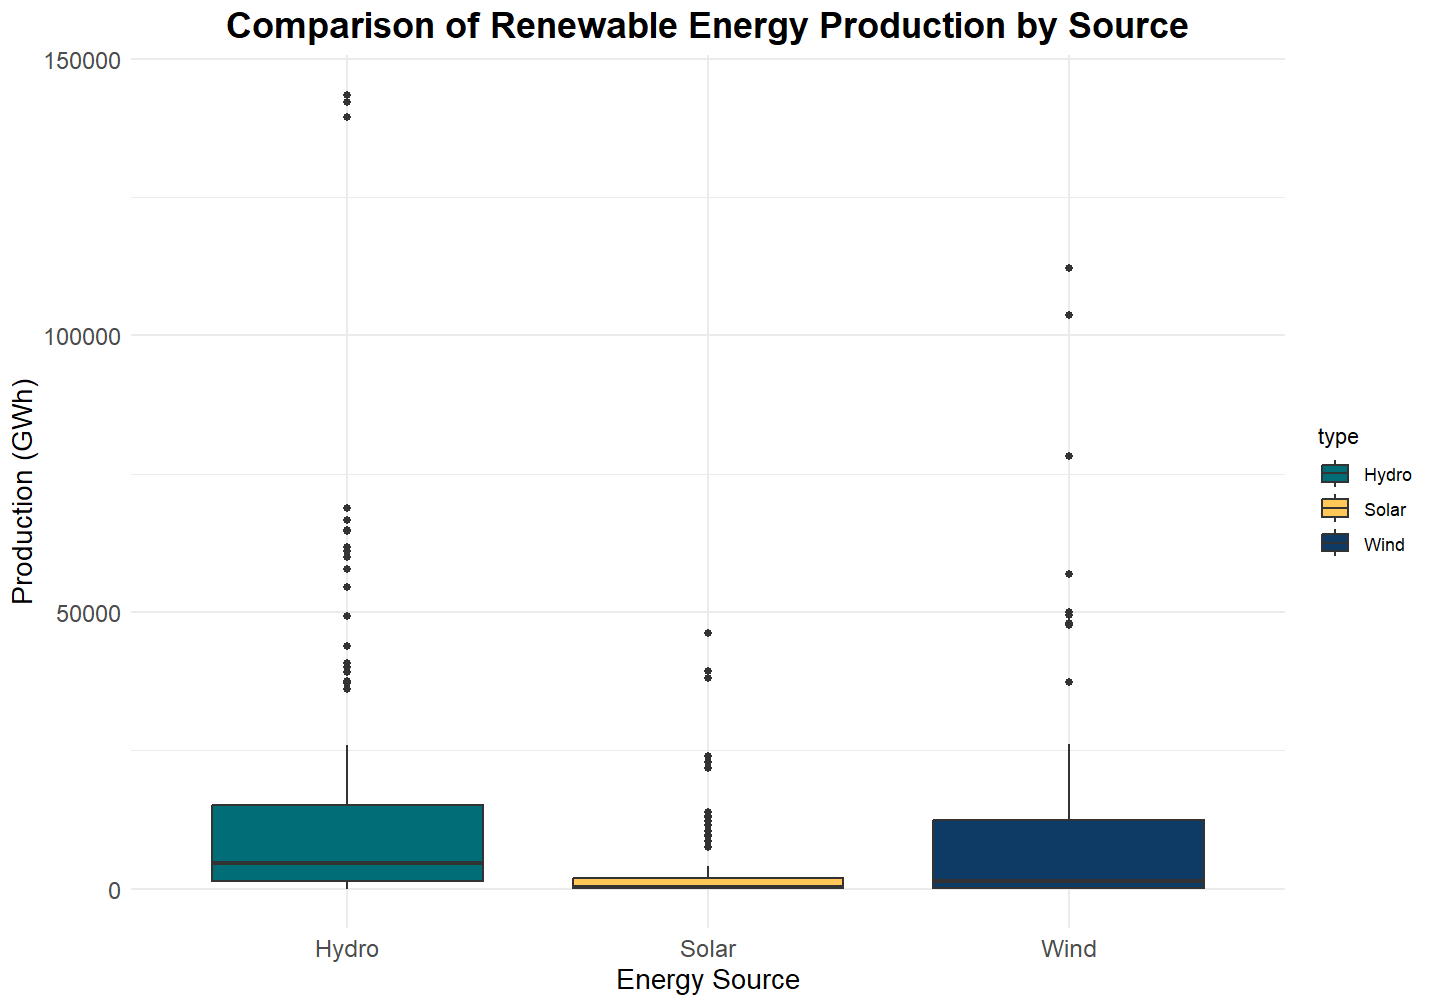
\includegraphics{../images/box_plot.png}

}

\caption{Energy Production Boxplot}

\end{figure}%

As you can see, much of the data lies on the lower end of the boxplot,
highlighting that there are a few ``outliers'' that account for vastly
more energy production than even the rest of the top 1/4 producers. This
is true for each of the three types of renewable energy being tracked.

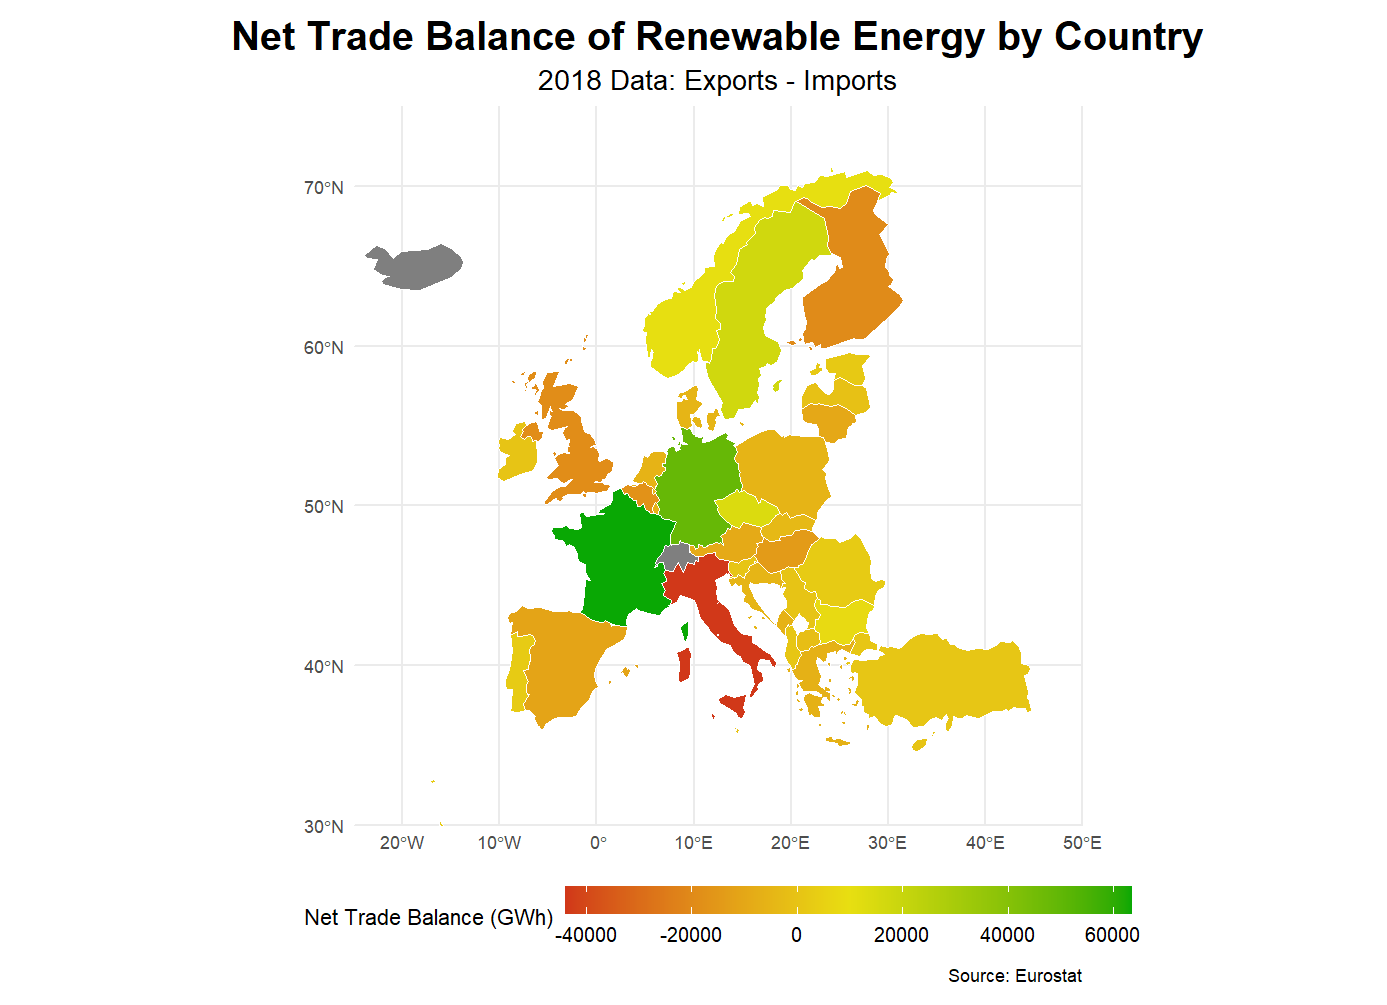
\includegraphics{../images/net_trade_map.png} This color-coded map
displays which countries in the EU contribute and benefit most from
power sharing. At the top of the charts is France, and what looks to be
the most reliant on outside energy is Italy. This visualization provides
a purely visual insight into the way that power is distributed among
countries, and which countries are ``sucklers'' on the European power
grid.

This visualization provides key insights into the steps that individual
countries are taking towards self-sustaiment as well as moving towards
renewable energy. Naturally the shift to renewable energy is something
that will take quite some time, and data visualization like this will
allow us to better track the progress of countries.

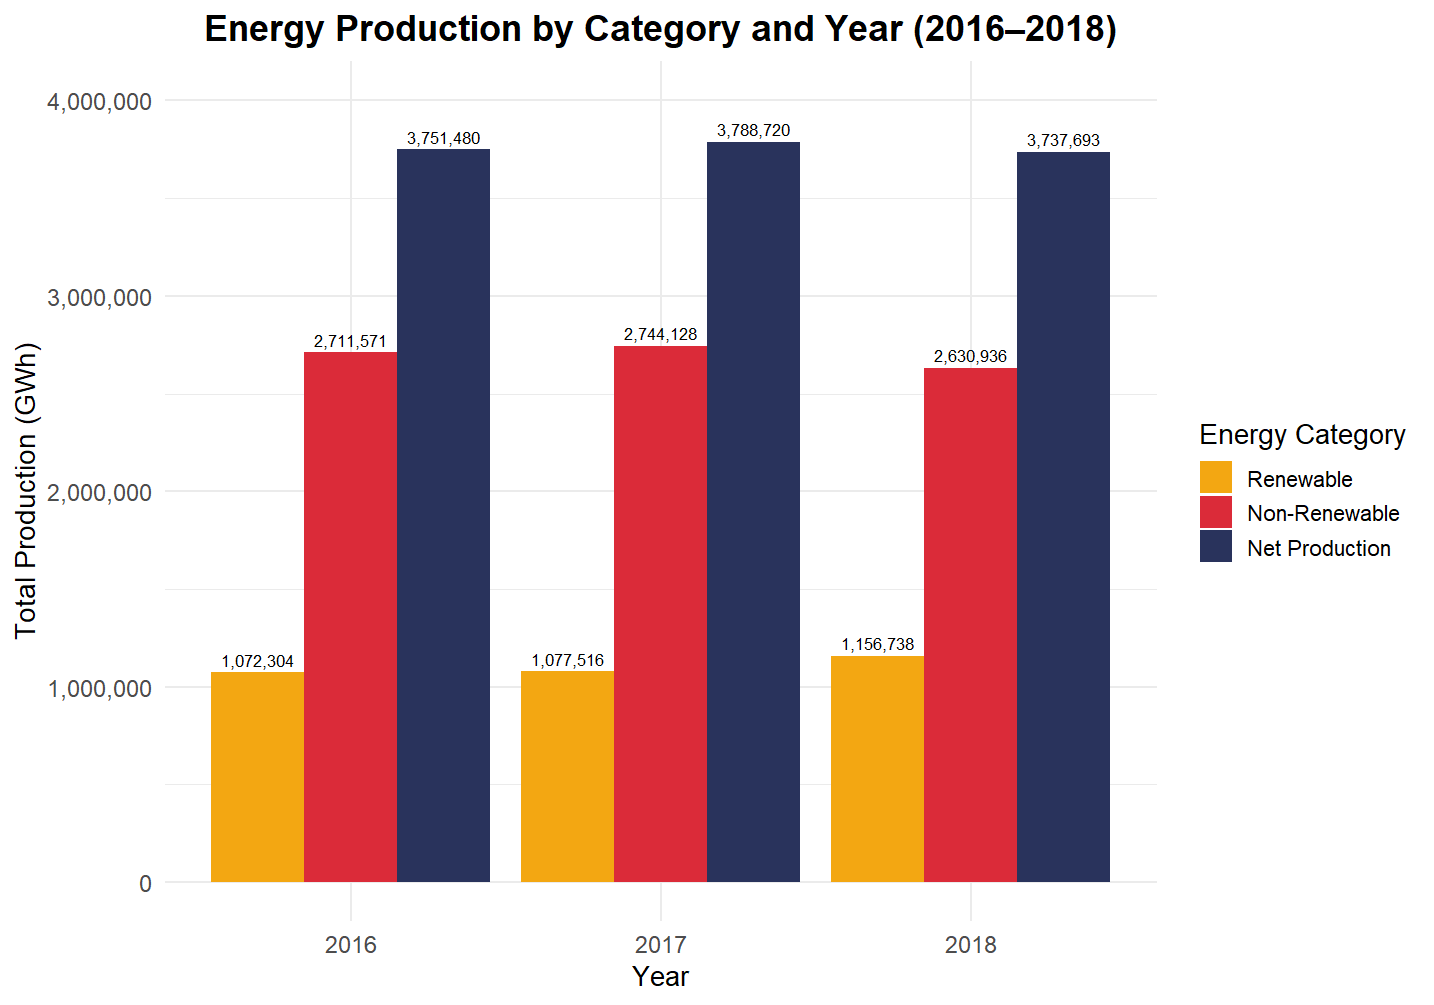
\includegraphics{../images/energy_category_years.png} Attached above is
a bar chart of energy production across the years 2016-2018. You can see
that there is an increase in renewable energy production across the
three years, signifying more of an emphasis being placed on renewable
energy. However, the visualization provides more insight than just that.
The increase in renewable energy from 2016 to 2017 is a mere
\textasciitilde5,000 GWh, but the increase in renewable energy
production from 2017 to 2018 is \textasciitilde77,000 GWh. This shows
that not onlt is there an increase in production of renewable energy,
the rate at which countries are switching to renewable energy is ALSO
increasing! This is good to see, that the switch to renewable energy is
actually picking up steam. Early reports show that this trend is still
being followed, although that data is outside of the scope of this
report.

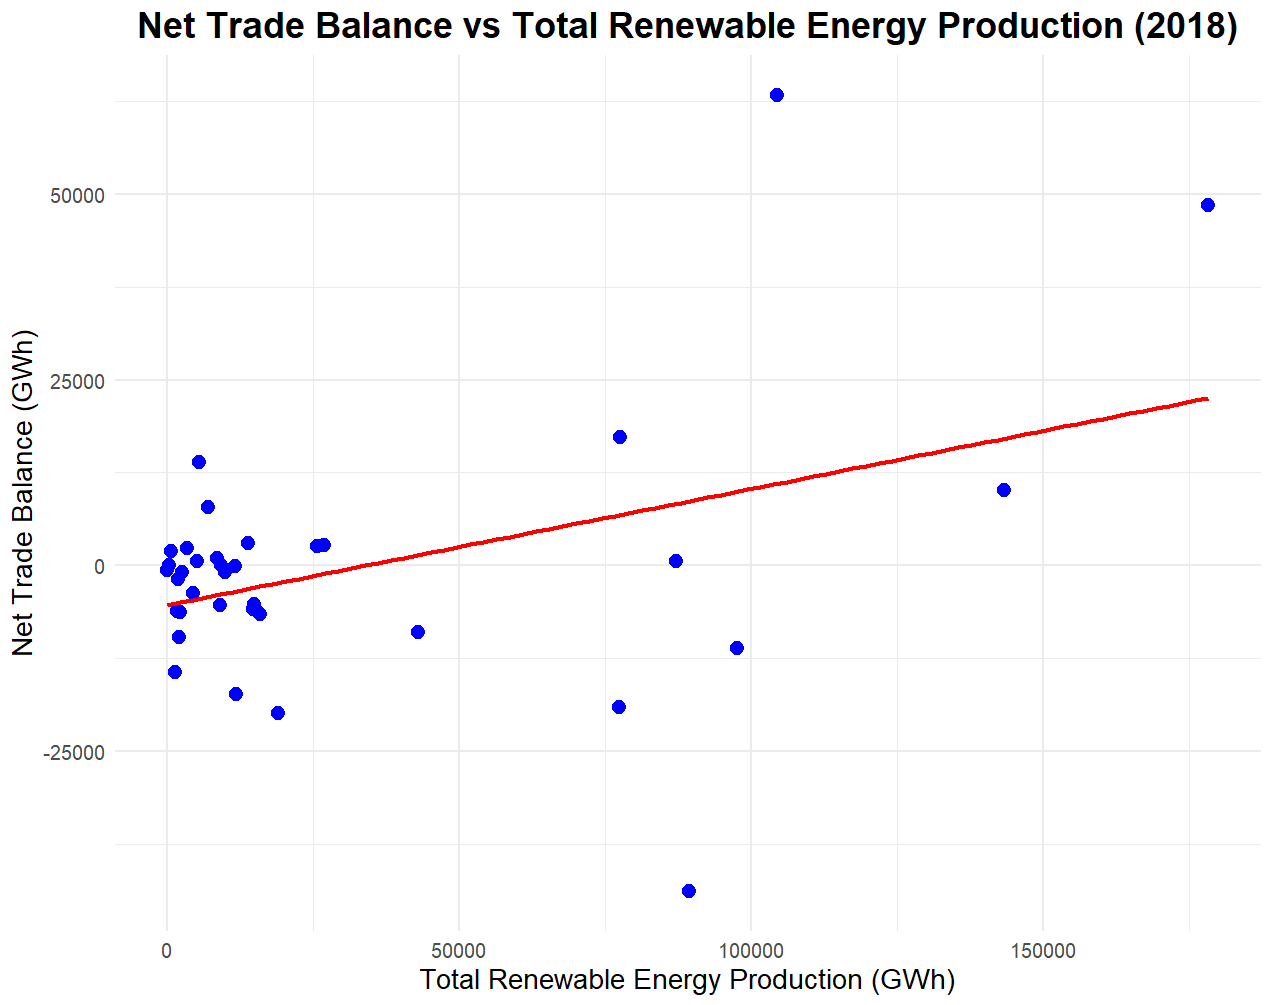
\includegraphics{../images/corr_net_trade_energy.png} This is perhaps
one of the most profound findings of the study. Although the coefficient
of correlation is relatively weak, there is in fact a correlation
between countries that generate enough power to have a surplus, and
countries that produce more renewable energy. This has already taken
into account the proportions of renewable vs total energy production.
Naturally, this is not a purely causative relationship, as there are
many other factors to take into account, such as GDP, Leadership, and
other factors that may confound this correlation, but the data shows
that countries that produce more renewable energy tend to have a surplus
of energy, hinting at its effectiveness and necessity going forward in
the journey to a more renewable power grid.

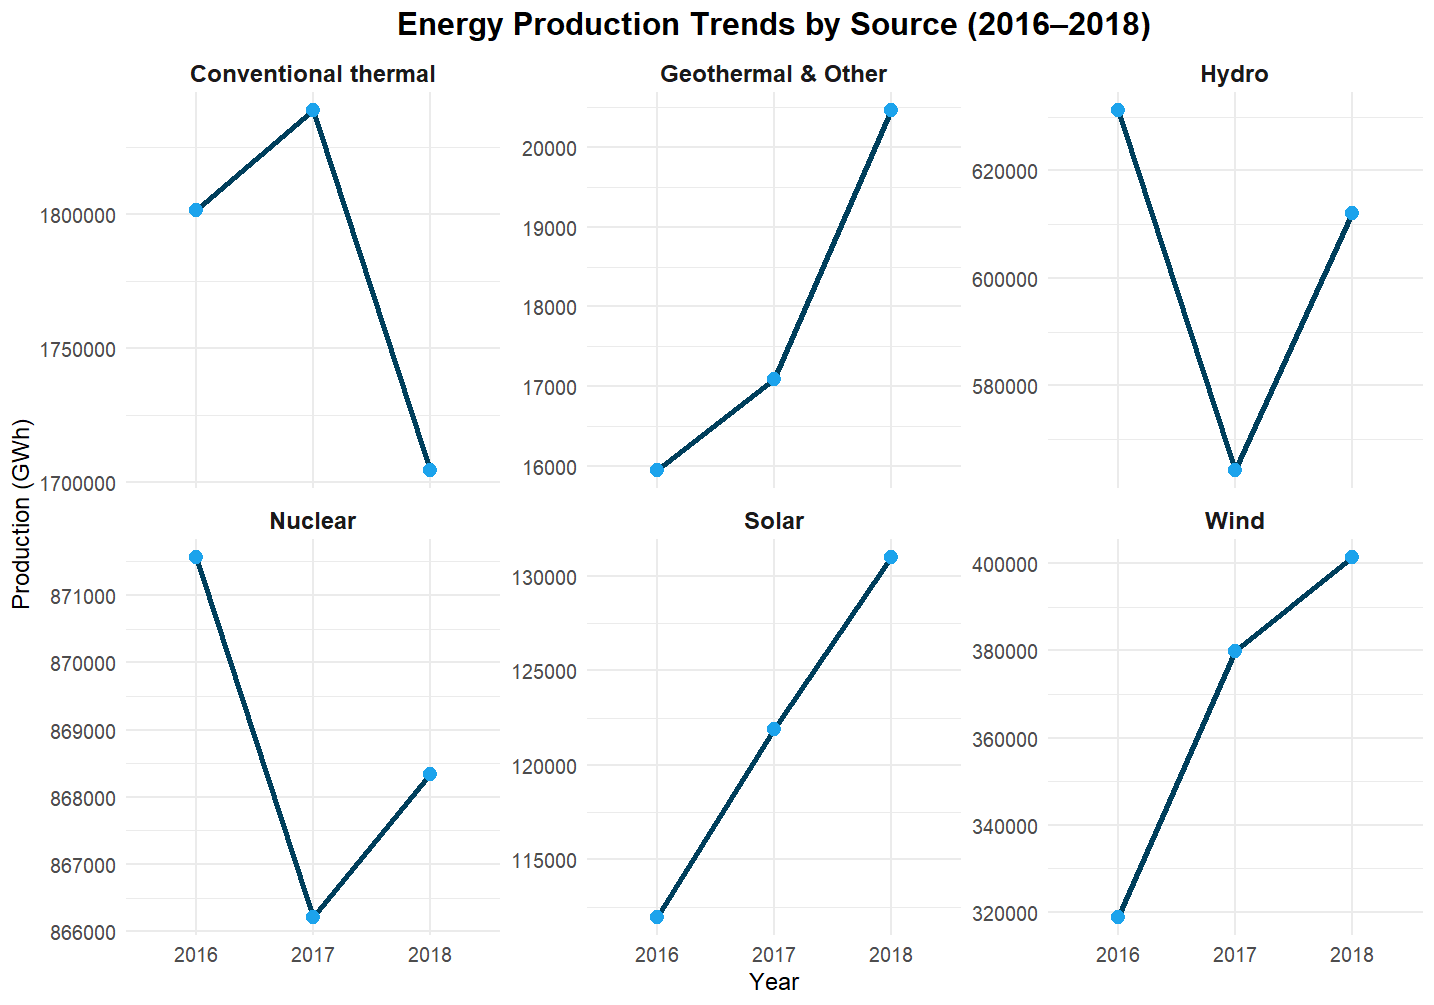
\includegraphics{../images/energy_trends.png} This is another very
interesting visual. This graphic provides insight not only into the
amount of each kind of energy being produced, but also highlights the
ways in which their production is changing, such as the ``geothermal /
other'' seeing a sharp uptick from 2017 to 2018, or the dip and recovery
that was experienced by both nuclear and Hydro energy. While surely
there are many many factors that influence how much of a certain power
type is produced, this visual gives an insight into the short-term
trends of the energy production types. That is to say, this gives us
insight into the ``What'' but not necessarily the ``Why''

\begin{verbatim}
# A tibble: 8 x 4
  type                 Total_2016 Total_2017 Totat_2018
  <chr>                     <dbl>      <dbl>      <dbl>
1 Conventional thermal   1801452.   1838783.   1704429.
2 Geothermal               10282.     11395.     12444.
3 Hydro                   631264.    564250.    611994.
4 Nuclear                 871560.    866212.    868334.
5 Other                     5670.      5692.      8019.
6 Pumped hydro power       32889.     33444.     50154.
7 Solar                   111948.    121911.    130968.
8 Wind                    318810.    379965.    401332.
\end{verbatim}

\begin{longtable}[]{@{}llll@{}}
\toprule\noalign{}
Type of Energy & 2016 Total & 2017 Total & 2018 Total \\
\midrule\noalign{}
\endhead
\bottomrule\noalign{}
\endlastfoot
Conventional Thermal & 1,801,451.654 & 1838783.375 & 1704429.420 \\
Geothermal & 10,281.953 & 11,394.997 & 12,443.754 \\
Hydro (traditional) & 631,263.647 & 564,249.938 & 611,993.531 \\
Nuclear & 871,560.205 & 866,211.980 & 868,333.983 \\
Hydro (pumped) & 32,889.277 & 33,443.817 & 50,153.928 \\
Solar & 111,948.354 & 121,910.507 & 130,968.490 \\
Wind & 318,809.583 & 379,964.520 & 401,332.380 \\
Other & 5,670.308 & 5,692.438 & 8,109.144 \\
\end{longtable}

Provide an overview of the main insights you found from the data.
Include multiple visualizations (e.g., graphs, tables, maps) to help
explain the data. Ensure to include a table that summarizes key
statistics, and at least one graph/plot. Explain each visualization in
the narrative (e.g., what trends the graph shows, what the table tells
us about the data). Optional: Create a map if it adds value to your
analysis.~

\subsection{6. Analysis of Research
Questions~}\label{analysis-of-research-questions}

\paragraph{1. How does the total energy production vary across European
countries in 2018? Which are the top 5 most produced
?}\label{how-does-the-total-energy-production-vary-across-european-countries-in-2018-which-are-the-top-5-most-produced}

Answering this question is important because it gives a better view of
what energy security in the European Union looks like. In the event of a
disaster that takes out the energy production stations of a certain
country, how tolerant is that country, as well as the rest of the
european union, to the fluctuations in power availability that may
occur? \#\#\#\# 2. What is the proportion of energy production for the
European countries in 2018?

This is an important question to answer because it allows to get a
better read into the energy ``leadership'' of a country, ie. which
countries are ``leading the charge'' in energy production. This likely
corresponds to bargaining power in the continental stage, as energy is
one of the most important commodities for a country to have.

\paragraph{3. How have renewable energy trends changed over time
(2016--2018) for European countries? (Line
chart)}\label{how-have-renewable-energy-trends-changed-over-time-20162018-for-european-countries-line-chart-1}

Answering this question is key to gauging how close the European union
is to it's sustainable energy goals. Regardless of actual renewable
energy production, we are able to see the rate at which countries are
making a shift to renewable energy, which serves as a marker of whether
or not a country is on track to meet the goals set by and for them, in
terms of renewable energy. This is especially important when considering
how much of a push the EU is making towards renewable energy. Discuss
how your data addresses each research question. Analyze the results with
the help of the visualizations and any relevant statistics. Use
narrative text to provide context and explain what the visualizations
reveal about the data.~

\subsection{7. Additional Analysis
(Optional)~}\label{additional-analysis-optional}

If applicable, apply more advanced statistical methods (e.g., hypothesis
testing, regression analysis, ANOVA) to provide further insights.
Mention any trends or anomalies discovered in the data and discuss their
implications.~

\subsection{8. Conclusion~}\label{conclusion}

Summarize the findings from your analysis. Answer each research question
based on the results. Discuss any limitations in your analysis and
suggest areas for future research or analysis.~

The analysis of European energy production from 2016 to 2018 highlights
a significant shift towards renewable energy, driven by the EU's
commitment to sustainability and reduced carbon emissions. While nuclear
and thermal energy still dominate, wind energy production rose by 34.2\%
between 2016 and 2017 and another 13.8\% from 2017 to 2018, illustrating
rapid growth. Similarly, solar energy production increased by 10.7\% and
11.6\% year-over-year, showing consistent adoption. Major contributors
like France and Germany, which accounted for significant portions of
total production, underscore regional disparities, as smaller nations
contribute far less. The findings underscore progress in renewable
energy adoption while highlighting the importance of continued
investment and policy support for a sustainable energy future.

Research Questions:

1.⁠ ⁠How have renewable energy trends evolved across European countries
between 2016 and 2018? 2.⁠ ⁠What factors contribute to the disparities in
energy production across EU member states?

Limitations:

1.⁠ ⁠The analysis relies on Eurostat data, which may have reporting
inconsistencies or gaps for certain countries. 2.⁠ ⁠The study focuses on
production data, leaving out consumption patterns or economic impacts of
the energy transition.

\paragraph{1. How does the total energy production vary across European
countries in 2018? Which are the top 5 most produced
?}\label{how-does-the-total-energy-production-vary-across-european-countries-in-2018-which-are-the-top-5-most-produced-1}

In 2018, total energy production varied substantially across European
countries, largely depending on their resource availability,
infrastructure, and policy focus. France, Germany, the United Kingdom,
Italy, and Spain emerged as the top five energy producers, with France
notably leading due to its extensive nuclear capacity and Germany
following closely with a more diversified energy mix.

\paragraph{2. What is the proportion of energy production for the
European countries in
2018?}\label{what-is-the-proportion-of-energy-production-for-the-european-countries-in-2018}

The proportion of energy production was unevenly distributed, with a few
large economies dominating the output. France held a significant share,
followed by Germany, while other countries produced comparatively
smaller proportions. Overall, a handful of major players accounted for
the bulk of Europe's total energy supply in 2018.

\paragraph{3. How have renewable energy trends changed over time
(2016--2018) for European
countries?}\label{how-have-renewable-energy-trends-changed-over-time-20162018-for-european-countries}

Between 2016 and 2018, renewable energy production in Europe increased
steadily, with wind and solar sources experiencing particularly strong
growth. Not only did the volume of renewable energy rise, but the rate
of growth also accelerated over this period, reflecting the EU's
strengthening commitment to reducing fossil fuel dependence and
achieving sustainability targets.

\subsection{9. References~}\label{references}

\url{https://ec.europa.eu/eurostat/statistics-explained/index.php?title=Archive:Electricity_generation_statistics_\%E2\%80\%93_first_results}

\url{https://github.com/rfordatascience/tidytuesday/blob/main/data/2020/2020-08-04/Electricity_generation_statistics_2019.xlsx}

\url{https://github.com/rfordatascience/tidytuesday/blob/main/data/2020/2020-08-04/readme.md}

Cite any sources used in your report (data, articles, books) following
your chosen citation style (e.g., APA7, MLA9). If you are using data
from an external source like Eurostat or OECD, make sure to properly
cite these sources.~

\subsection{10. Appendix: Code~}\label{appendix-code}

Include an appendix where all code used for the analysis is placed. Code
should be included in the appendix only and should not be mixed in the
main body of the report. Include a code style guide at the top of the
code section.




\end{document}
